\chapter{التفاعلات بين الأنواع}\label{ch:b1:species-interactions}

في سنة 1963، على شاطئ صخري في المحيط الهادئ، بدأ عالم بيئة شاب
يرمي كل نجم بحر يجده على امتداد من الصخر عائدًا إلى
البحر، وظل يفعل ذلك سنوات. وكان نجم البحر يأكل بلح البحر. فبلا
نجوم بحر انتشر بلح البحر نازلًا على الصخر وزاحم البرنقيل
والبطلينوس والكيتونات والطحالب التي كانت تعيش هناك؛ فهبط مجتمع من
خمسة عشر نوعًا إلى ثمانية. فمفترس واحد، ليس هو نفسه وفيرًا ولا
كبيرًا، كان يمسك التجمع كله في مكانه. فالأنواع لا تتقاسم مكانًا
فحسب؛ بل تتنافس عليه، ويأكل بعضها بعضًا، وتعيش داخل بعضها وعليه،
ويعتمد بعضها على بعض، والمجتمع مجموع هذه التفاعلات. ويصنّف هذا
الفصل تلك التفاعلات، ويعطي النماذج الكمية \omterm{def:b1:species-interactions:types}{للتنافس} \omterm{def:b1:species-interactions:types}{والافتراس} التي
تحتملها سنة أولى، ويبيّن بالتجارب كيف يستطيع تفاعل واحد أن يشكّل
نظامًا بيئيًا كاملًا.

\section{تصنيف للتفاعلات}

\begin{definition}[التفاعلات بين الأنواع]\label{def:b1:species-interactions:types}
\index{تنافس}\index{افتراس}\index{تطفل}\index{تقايض}\index{معايشة}
يُصنَّف التفاعل بين نوعين بأثره في
كل منهما: $+$ (نفع)، أو $-$ (ضرر)، أو $0$. وفي \emph{التنافس} ($-/-$) يستعمل
كلاهما موردًا شحيحًا. و\emph{الافتراس} ($+/-$): يقتل أحدهما
الآخر ويأكله؛ و\emph{أكل العشب} ($+/-$) حين يكون المأكول نباتًا
وينجو عادة؛ و\emph{التطفل} ($+/-$) حين يعيش المستغِلّ
على مضيف أو فيه ولا يقتله فورًا. و\emph{التقايض}
($+/+$): ينتفع كلاهما. و\emph{المعايشة} ($+/0$): ينتفع أحدهما،
ولا يتأثر الآخر. و\emph{التضادّ} ($-/0$): يتضرر أحدهما،
ولا يتأثر الآخر. وكل تفاعل ضغط انتخابي على الشريكين
معًا، وتكيّفهما المتبادل عبر الأجيال هو
\emph{التطور المشترك}.
\end{definition}

\begin{example}[شجرة واحدة، والستة كلها]\label{ex:b1:species-interactions:oak}
البلوطة \omterm{def:b1:species-interactions:types}{تنافس} جاراتها على الضوء؛ ويأكل بلوطها
القيقُ (\omterm{def:b1:species-interactions:types}{افتراس}) وتأكل أوراقها اليرقات (أكل عشب)؛ ويسحب الدبق
عصارتها (\omterm{def:b1:species-interactions:types}{تطفل})؛ وتبادل جذورها \omterm{def:b1:carbohydrates:monosaccharide}{السكاكر} بالفوسفات
مع فطر (\omterm{def:b1:species-interactions:types}{تقايض})؛ وتنمو السرخسيات على قشرتها، لا تستعملها إلا
مجثمًا (\omterm{def:b1:species-interactions:types}{معايشة})؛ ويقتل ظلها العشب تحتها
(تضادّ).
\end{example}

\section{التنافس}

\begin{definition}[التنافس بين الأنواع]\label{def:b1:species-interactions:competition}
\index{إقصاء تنافسي}\index{تقاسم المكانات}\index{إزاحة صفاتية}
يتنافس نوعان حين يستعملان كلاهما موردًا --- غذاءً أو ضوءًا أو
ماءً أو مكانًا أو مواضع تعشيش --- يحدّ إمدادُه نموَّهما.
وقد يكون \omterm{def:b1:species-interactions:types}{التنافس} \emph{استغلالًا} (كل واحد يأخذ ما كان الآخر
سيستعمله) أو \emph{تداخلًا} (عدوان مباشر، أو سموم،
أو حمى). ونتيجته تتبع \emph{مبدأ الإقصاء
\omterm{def:b1:enzymes:inhibitors}{التنافسي}}: فنوعان يحتاجان إلى المورد الحادّ نفسه بالطريقة
نفسها لا يستطيعان التعايش إلى ما لا نهاية في بيئة ثابتة؛
فالمنافس الأفضل يقصي الآخر. ولذلك يختلف المتنافسون المتعايشون
في \omterm{def:b1:ecosystem-organization:niche}{المكانة} (\emph{تقاسم \omterm{def:b1:ecosystem-organization:niche}{المكانات}}) --- وحيث يتداخل نوعان
كثيرًا ما يتباعدان في الشكل أكثر مما يفعلان حيث يعيش كل واحد
وحده (\emph{الإزاحة الصفاتية}).
\end{definition}

\begin{proposition}[نموذج لوتكا-فولتيرا للتنافس]\label{prop:b1:species-interactions:lotka}
لينمُ نوعان نموًا لوجستيًا (\cref{ch:b1:populations}) وليُحسب
كل فرد من النوع 2 بمنزلة $\alpha$ فردًا من النوع
1 في استعمال مورد النوع 1، وكل فرد من النوع 1 بمنزلة $\beta$
من النوع 2:
\[
\frac{\dd N_1}{\dd t} = r_1 N_1\left(1 - \frac{N_1 + \alpha N_2}{K_1}\right),
\qquad
\frac{\dd N_2}{\dd t} = r_2 N_2\left(1 - \frac{N_2 + \beta N_1}{K_2}\right).
\]
يكفّ النوع 1 عن النمو على الخط $N_1 + \alpha N_2 = K_1$ (وهو
\emph{خط تساويه}\index{خط تساوٍ})، والنوع 2 على $N_2 + \beta N_1 = K_2$.
فإذا كان كل نوع يحدّ نفسه أكثر مما يحدّ الآخر ($\alpha <
K_1/K_2$ و$\beta < K_2/K_1$) تقاطع الخطان وكان توازن
النوعين مستقرًا و\emph{تعايشا}؛ وإذا وقع أحد الخطين
كله فوق الآخر \emph{أقصى} ذلك النوع الآخرَ دائمًا؛
وإذا كان كل واحد يحدّ الآخر أكثر مما يحدّ نفسه توقف الفائز
على الأعداد الابتدائية.
\end{proposition}
\begin{proof}[برهان جزئي]
ينمو النوع 1 تحت \omterm{prop:b1:species-interactions:lotka}{خط تساويه} ويتراجع فوقه؛ وكذلك النوع 2.
وحين يتقاطع الخطان مع وقوع خط النوع 1 فوق خط النوع
2 على محور $N_1$ وتحته على محور $N_2$، تُردّ أي نقطة خارج
التقاطع إليه من كل جانب: فالتقاطع
توازن مستقر بحضور النوعين معًا. وحين يقع خط النوع 1
كله خارج خط النوع 2، تكون كل نقطة يستطيع فيها النوع
2 أن ينمو نقطةً ينمو فيها النوع 1 أيضًا ويظل ينمو
بعد أن يتوقف النوع 2، حتى يبلغ $K_1$ عند
$N_2 = 0$. والتحليل الكامل في كتاب السنة الثانية؛ ورسم
الخطين يعطي كل النتائج دونه.
\end{proof}

\begin{omfigure}
\begin{tikzpicture}[font=\footnotesize, >=Stealth, line cap=round]
  \begin{scope}
    \draw[->, thick] (0,0) -- (4.6,0) node[below left] {$N_1$};
    \draw[->, thick] (0,0) -- (0,4.4) node[below right] {$N_2$};
    \draw[very thick, omDef] (4.0,0) -- (0,3.0) node[pos=0.15, above right, omDef!80!black] {النوع 1 يتوقف};
    \draw[very thick, omThm] (2.6,0) -- (0,4.0) node[pos=0.85, right, omThm!80!black] {النوع 2 يتوقف};
    \fill (1.63,1.78) circle (2pt); \node[anchor=west] at (1.75,1.95) {تعايش مستقر};
    \draw[->, gray] (3.6,3.0) -- (2.2,2.2); \draw[->, gray] (0.4,0.4) -- (1.3,1.4);
    \node[anchor=north] at (2.3,-0.8) {كل نوع يحدّ نفسه أكثر};
  \end{scope}
  \begin{scope}[xshift=7.2cm]
    \draw[->, thick] (0,0) -- (4.6,0) node[below left] {$N_1$};
    \draw[->, thick] (0,0) -- (0,4.4) node[below right] {$N_2$};
    \draw[very thick, omDef] (4.0,0) -- (0,4.0) node[pos=0.5, above right, omDef!80!black] {النوع 1 يتوقف};
    \draw[very thick, omThm] (2.4,0) -- (0,2.4) node[pos=0.35, anchor=north east, align=right, omThm!80!black] {النوع 2\\ يتوقف};
    \fill (4.0,0) circle (2pt); \node[anchor=north, font=\scriptsize] at (3.5,-0.3) {النوع 1 وحده عند $K_1$};
    \draw[->, gray] (1.0,3.4) -- (2.1,2.3); \draw[->, gray] (2.4,2.0) -- (3.4,0.7);
    \node[anchor=north] at (2.3,-0.8) {النوع 1 يفوز في كل مكان};
  \end{scope}
\end{tikzpicture}

{\small نتيجتان من \omterm{def:b1:species-interactions:types}{تنافس} نوعين، تُقرآن من
\omterm{prop:b1:species-interactions:lotka}{خطي التساوي} (وهما الخطان اللذان يتوقف عندهما نمو كل نوع). يسارًا:
يتقاطع الخطان بحيث يكون كل نوع مكبوحًا بنفسه أكثر
مما يكبحه الآخر، فيتعايشان. ويمينًا: خط النوع 1
يقع خارج خط النوع 2، فيفوز النوع 1 دائمًا.}
\end{omfigure}

\begin{proposition}[الإقصاء التنافسي]\label{prop:b1:species-interactions:gause}
\index{مبدأ غوز}
نوعان يتنافسان على مورد حادّ واحد في بيئة ثابتة
لا يستطيعان الدوام معًا: فالذي تستطيع جمهرته أن تظل
تنمو عند مستوى مورد أدنى يدفع المورد دون ما
يحتاج إليه الآخر، فيتراجع الآخر إلى الانقراض.
\end{proposition}
\begin{proof}[شواهد]
نمّى غوز (1934) نوعين من الهدبيات، هما \emph{Paramecium aurelia}
و\emph{P.~caudatum}، على حصة يومية من البكتيريا. فكل واحد منهما
وحده نما نموًا لوجستيًا إلى هضبته. وأما معًا فبلغ \emph{P.~aurelia}،
وهو ينمو أسرع ويحتاج إلى غذاء أقل للفرد، هضبتَه
تقريبًا بينما تراجع \emph{P.~caudatum} إلى العدم في ستة عشر
يومًا. ونوع ثالث، هو \emph{P.~bursaria}، يتغذى في قاع
الأنبوب حيث لا يتغذى \emph{P.~aurelia}، تعايش معه
إلى ما لا نهاية: فلم يقع الإقصاء إلا حين تطابقت المكانتان.
\end{proof}

\begin{omfigure}
\begin{tikzpicture}
\begin{axis}[
  width=0.8\linewidth, height=6.2cm,
  axis x line=bottom, axis y line=left,
  xmin=0, xmax=20, ymin=0, ymax=220,
  xlabel={الأيام}, ylabel={أفراد في \qty{0.5}{mL}},
  xlabel style={font=\small}, ylabel style={font=\small},
  tick label style={font=\small},
  legend style={font=\scriptsize, at={(0.98,0.02)}, anchor=south east, draw=none, fill=none},
  legend cell align=left,
]
\addplot[omDef, very thick, dashed, domain=0:20, samples=60] {200/(1+40*exp(-0.8*x))};
\addlegendentry{\emph{P.~aurelia} وحده}
\addplot[omThm, very thick, dashed, domain=0:20, samples=60] {130/(1+25*exp(-0.55*x))};
\addlegendentry{\emph{P.~caudatum} وحده}
\addplot[omDef, very thick, domain=0:20, samples=60] {170/(1+40*exp(-0.65*x))};
\addlegendentry{\emph{P.~aurelia} مخلوطًا}
\addplot[omThm, very thick, domain=0:20, samples=80] {80*exp(-0.05*(x-6)^2)*(x<12) + 80*exp(-0.05*36)*exp(-0.5*(x-12))*(x>=12)};
\addlegendentry{\emph{P.~caudatum} مخلوطًا}
\end{axis}
\end{tikzpicture}

{\small تجربة غوز في \omterm{def:b1:species-interactions:types}{التنافس} (معادة الرسم عن معطياته).
كل نوع وحده ينمو إلى هضبته؛ ومعًا يرتفع \emph{P.~aurelia}
إلى هضبته تقريبًا بينما يبلغ \emph{P.~caudatum} ذروة ثم يُساق
إلى الانقراض.}
\end{omfigure}

\begin{example}[إزاحة صفاتية في العصافير]\label{ex:b1:species-interactions:finches}
في الجزر التي يعيش فيها عصفور أرضي واحد وحده يكون منقاره متوسط
الحجم؛ وحيث يتقاسم نوعان جزيرة يكون منقاراهما
أصغر وأكبر على الترتيب مما لكل واحد منهما وحده، وقد انزاح كل نوع
نحو بذور لا يستطيع الآخر كسرها. فقد قسم التطور المكانتين،
والقسمة مرئية في المنقار.
\end{example}

\section{الافتراس وأكل العشب}

\begin{definition}[الاستجابة الوظيفية]\label{def:b1:species-interactions:functional}
\index{استجابة وظيفية}\index{زمن معالجة}
\emph{الاستجابة الوظيفية} لمفترس هي عدد الفرائس التي يأكلها
مفترس واحد في وحدة الزمن بدلالة كثافة الفريسة $N$.
وفي \emph{النمط I} تكون متناسبة مع $N$ (كالمرشِّح المغذي). و\emph{النمط II}:
يرتفع ثم يشبع، لأن كل فريسة تستغرق \emph{زمن معالجة}
$h$ لصيدها وأكلها وهضمها، لا يمكن خلاله أخذ غيرها.
و\emph{النمط III}: سيني --- منخفض عند الكثافة المنخفضة لأن المفترس
يتجاهل الفريسة النادرة أو لا يجدها، ثم يرتفع بحدة (وهو مفترس
يتحول إلى ما يكثر). و\emph{الاستجابة العددية} هي
تغير عدد المفترسات مع كثافة الفريسة، بالتكاثر
أو بالهجرة الداخلة.
\end{definition}

\begin{theorem}[معادلة الأقراص]\label{thm:b1:species-interactions:holling}
\index{معادلة الأقراص}
إذا بحث مفترس عند \emph{معدل هجوم} $a$ (المساحة الممسوحة في
وحدة الزمن، مضروبة في احتمال الأسر) وأنفق \omterm{def:b1:species-interactions:functional}{زمن معالجة}
$h$ على كل فريسة، كان عدد الفرائس المأخوذة لكل مفترس في وحدة
الزمن عند كثافة فريسة $N$ هو
\[
f(N) = \frac{aN}{1 + ahN} ,
\]
وهو يرتفع خطيًا بالمقدار $aN$ عند الكثافة المنخفضة ويشبع عند $1/h$ عند
الكثافة العالية؛ ويبلغ $f$ نصف أعظميته حين $N = 1/(ah)$. وفي الصورة
$1/f = 1/(aN) + h$ يكون رسم $1/f$ في مقابل $1/N$ خطًا مستقيمًا
ميلُه $1/a$ وتقاطعه $h$.
\end{theorem}
\begin{proof}
على مدى زمن كلي $T$ يبحث المفترس مدة $T_s$ ويعالج
الباقي. وهو باحثًا يلقى الفرائس بمعدل $aN$، فيكون العدد
المأسور $n = aN T_s$؛ ومعالجتها تأخذ $nh$، فيكون $T = T_s + nh =
n/(aN) + nh$، ومنه $n/T = aN/(1 + ahN)$. وحين $ahN \ll 1$ تكون المعالجة
مهملة و$f \approx aN$؛ وحين $ahN \gg 1$ لا يفعل المفترس
شيئًا غير المعالجة و$f \to 1/h$. وقلب المعادلة يعطي الصورة الخطية.
\end{proof}
\begin{proof}[شواهد]
جعل هولينغ (1959) مساعدًا معصوب العينين «يفترس» بطرف إصبعه
أقراصًا من ورق السنفرة منثورة على طاولة، يلتقط كل قرص يجده
(وهو \omterm{def:b1:species-interactions:functional}{زمن المعالجة}) قبل أن يعود إلى البحث؛ فأعطى عدد المُلتقَط في
الدقيقة في مقابل كثافة الأقراص هذا المنحني بالضبط، وأخذت المعادلة
اسمها من التجربة. والمفترسات الحقيقية --- فرس النبي على الذباب،
وسمكة شوكة الظهر على براغيث الماء --- تعطي الشكل نفسه، وأزمنة
معالجتها من ثوانٍ إلى ساعات.
\end{proof}

\begin{omfigure}
\begin{tikzpicture}
\begin{axis}[
  width=0.78\linewidth, height=6.2cm,
  axis x line=bottom, axis y line=left,
  xmin=0, xmax=100, ymin=0, ymax=12,
  xlabel={كثافة الفريسة $N$ (في \unit{m^2})}, ylabel={فرائس مأكولة لكل مفترس في اليوم},
  xlabel style={font=\small}, ylabel style={font=\small},
  tick label style={font=\small},
  legend style={font=\scriptsize, at={(0.98,0.03)}, anchor=south east, draw=none, fill=none},
  legend cell align=left,
]
\addplot[omExo!80!black, very thick, domain=0:100, samples=2] {0.1*x};
\addlegendentry{النمط I: $f = aN$}
\addplot[omDef, very thick, domain=0:100, samples=80] {0.5*x/(1+0.05*x)};
\addlegendentry{النمط II: $f = aN/(1+ahN)$، والهضبة $1/h = 10$}
\addplot[omThm, very thick, domain=0:100, samples=80] {10*x^2/(30^2+x^2)};
\addlegendentry{النمط III: سيني}
\draw[dashed, gray] (axis cs:0,10) -- (axis cs:100,10);
\end{axis}
\end{tikzpicture}

{\small الاستجابات الوظيفية الثلاث. النمط II يشبع عند $1/h$
(هنا عشر فرائس في اليوم، أي \omterm{def:b1:species-interactions:functional}{زمن معالجة} \qty{2.4}{h})؛ والنمط III
يبدأ ببطء لأن الفريسة النادرة تُغفَل.}
\end{omfigure}

\begin{proposition}[الدفاعات وسباق التسلح]\label{prop:b1:species-interactions:defences}
\index{محاكاة}\index{تلوين تحذيري}
تطوّر الفرائس والنباتات دفاعات --- التخفي، والدروع، والأشواك،
والسرعة، والسموم وألوانها المحذّرة (\emph{\omterm{prop:b1:species-interactions:defences}{التلوين التحذيري}})،
و\emph{المحاكاة}: نوع غير مؤذٍ ينسخ نوعًا سامًا (محاكاة بيتسية) أو
عدة أنواع سامة تتقارب على نمط واحد (محاكاة مولرية). وتدافع النباتات
عن نفسها بالأشواك والسيليكا والعفصيات والقلويدات
والغليكوزيدات السيانوجينية، وكثيرًا ما تستحثها الأضرار. وتطوّر
المفترسات وآكلات العشب إجراءات مضادة --- حواسّ أحدّ، \omterm{def:b1:enzymes:enzyme}{وإنزيمات}
مزيلة للسمية، ومقاومة للذيفان --- ويتطور الزوج معًا. والنتيجة
ليست إفناء الفريسة بل توازن جارٍ: فمفترس يأكل فريسته حتى
الانقراض يتبعها.
\end{proposition}

\begin{omfigure}
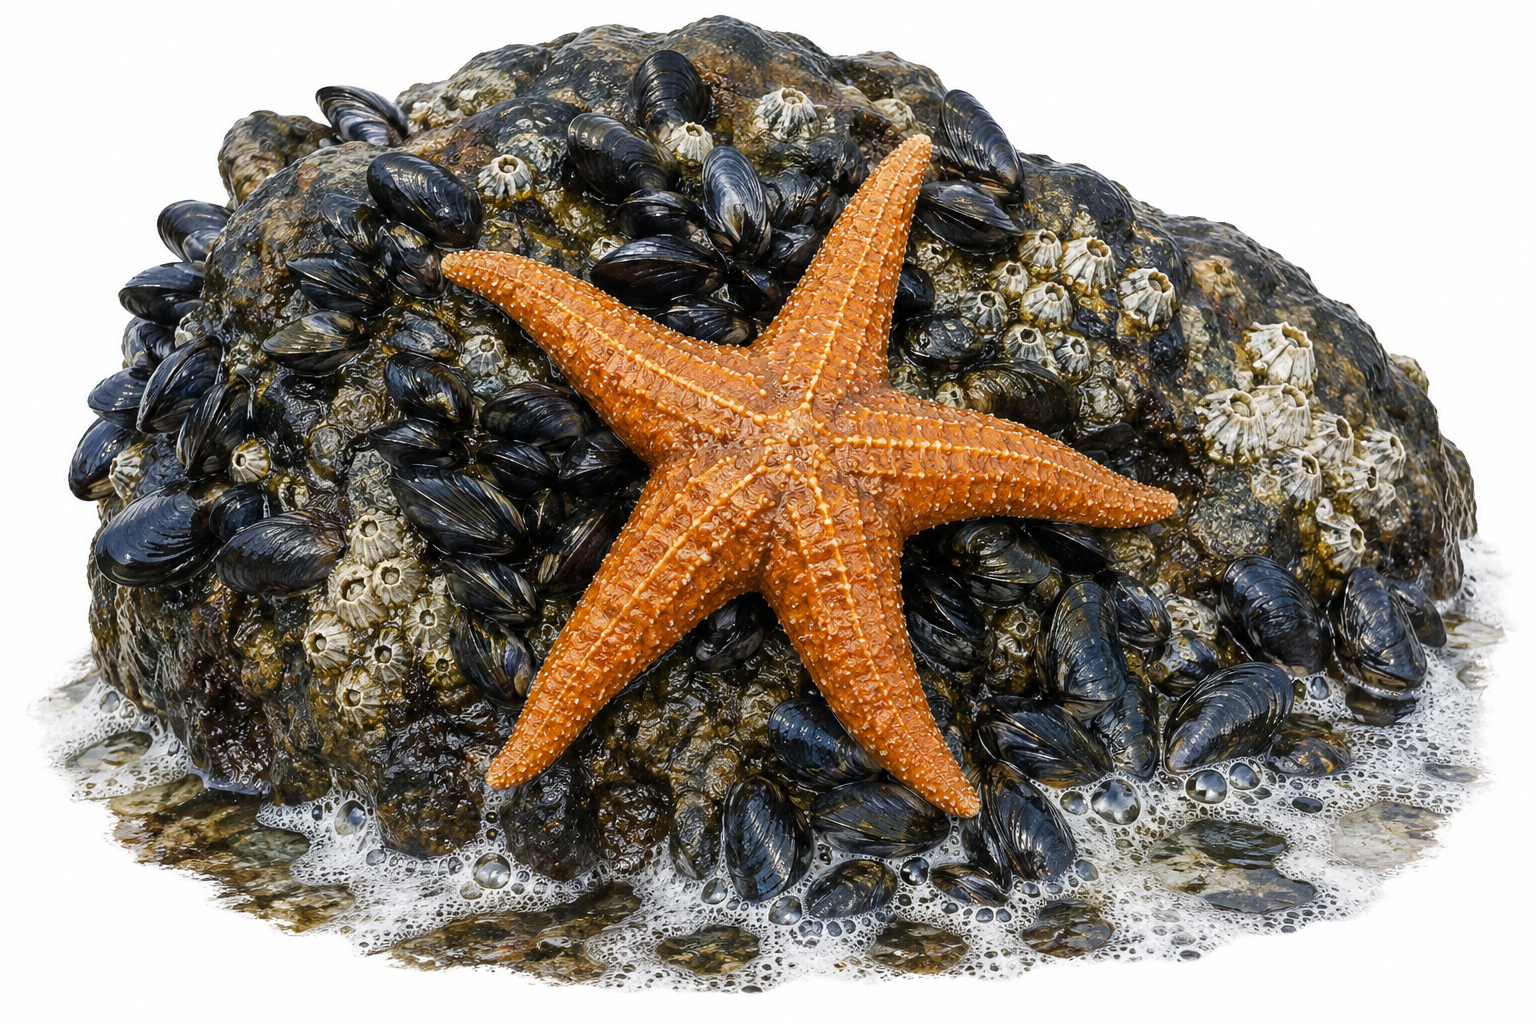
\includegraphics[width=0.6\linewidth]{images/book3/ai/b3-27-sea-star-mussels.png}

{\small نجم بحر مفترس على فراش من بلح البحر عند الجزر: وهو
المفترس المفتاح الذي حوّلت إزالتُه شاطئًا من خمسة عشر نوعًا إلى
أحادية زراعية من بلح البحر.}
\end{omfigure}

\section{العيش معًا: التطفل والتقايض والمعايشة}

\begin{definition}[التطفل والتكافل والتقايض]\label{def:b1:species-interactions:symbiosis}
\index{تكافل}\index{طفيلي}\index{أشنة}
\emph{الطفيلي} يعيش على حساب مضيف، عليه (طفيلي خارجي:
القراد، والقمل، والدبق) أو فيه (طفيلي داخلي: الشريطية، وطفيلي
الملاريا، وفطر الصدأ)، يأخذ المغذّيات ويخفض لياقته
دون أن يقتله بالضرورة؛ والطفيليات كثيرًا ما تكون متخصصة،
ذات دورات حياة معقدة عبر عدة مضيفين. و\emph{التكافل}
أي ارتباط وثيق دائم بين نوعين؛ و\emph{\omterm{def:b1:species-interactions:types}{التقايض}}
ارتباط ينتفع منه الاثنان: \omterm{def:b1:plant-water-minerals:mycorrhiza}{كالميكوريزا} (فطر على \omterm{def:b1:flowering-plant-organization:organs}{جذور}
نبات أو فيها، يبادل الفوسفات والماء بالسكر؛
\cref{ch:b1:plant-water-minerals})، \omterm{def:b1:plant-water-minerals:nodules}{والعقيدة الجذرية} (بكتيريا
مثبِّتة للنتروجين تطعمها البقولية)، و\emph{الأشنة} (فطر يؤوي
طحلبًا أو بكتيريا زرقاء)، ومرجان الشعاب (لاسع يؤوي
سوطيات دوّارة مركّبة ضوئيًا)، وجراثيم أمعاء المجترّ أو
النملة البيضاء (\cref{ch:b1:digestion-absorption})، والتلقيح (رحيق
مقابل نقل اللقاح). وكثير من أنواع \omterm{def:b1:species-interactions:types}{التقايض} بدأ تطفلًا أو
افتراسًا حوّله التطور المشترك للشريكين إلى منفعة متبادلة،
وتظل مشروطة: ففطر ميكوريزي في تربة غنية بالفوسفات
كلفةٌ، فيقلّله النبات.
\end{definition}

\begin{example}[التلقيح مقايضةً]\label{ex:b1:species-interactions:pollination}
تنفق الزهرة بضعة جولات من السكر على الرحيق؛ وتنفق النحلة طيرانًا
لجمعه وتحمل اللقاح بين الأزهار وهي تمضي. ولون
الزهرة ورائحتها وشكلها وتوقيتها موجّهة إلى ملقّحاتها،
وطول لسان النحلة ورؤيتها اللونية وذاكرتها في الاعتلاف
موجّهة إلى أزهارها؛ وبعض الأزواج مركّبة تركيبًا محكمًا ---
مهماز رحيق طويل والعثة الوحيدة التي يبلغه لسانها --- حتى إن أحدهما
لا يبقى بلا الآخر، وقد يعتمد مجتمع نباتي كامل على
بضعة أنواع من الحشرات.
\end{example}

\begin{omfigure}
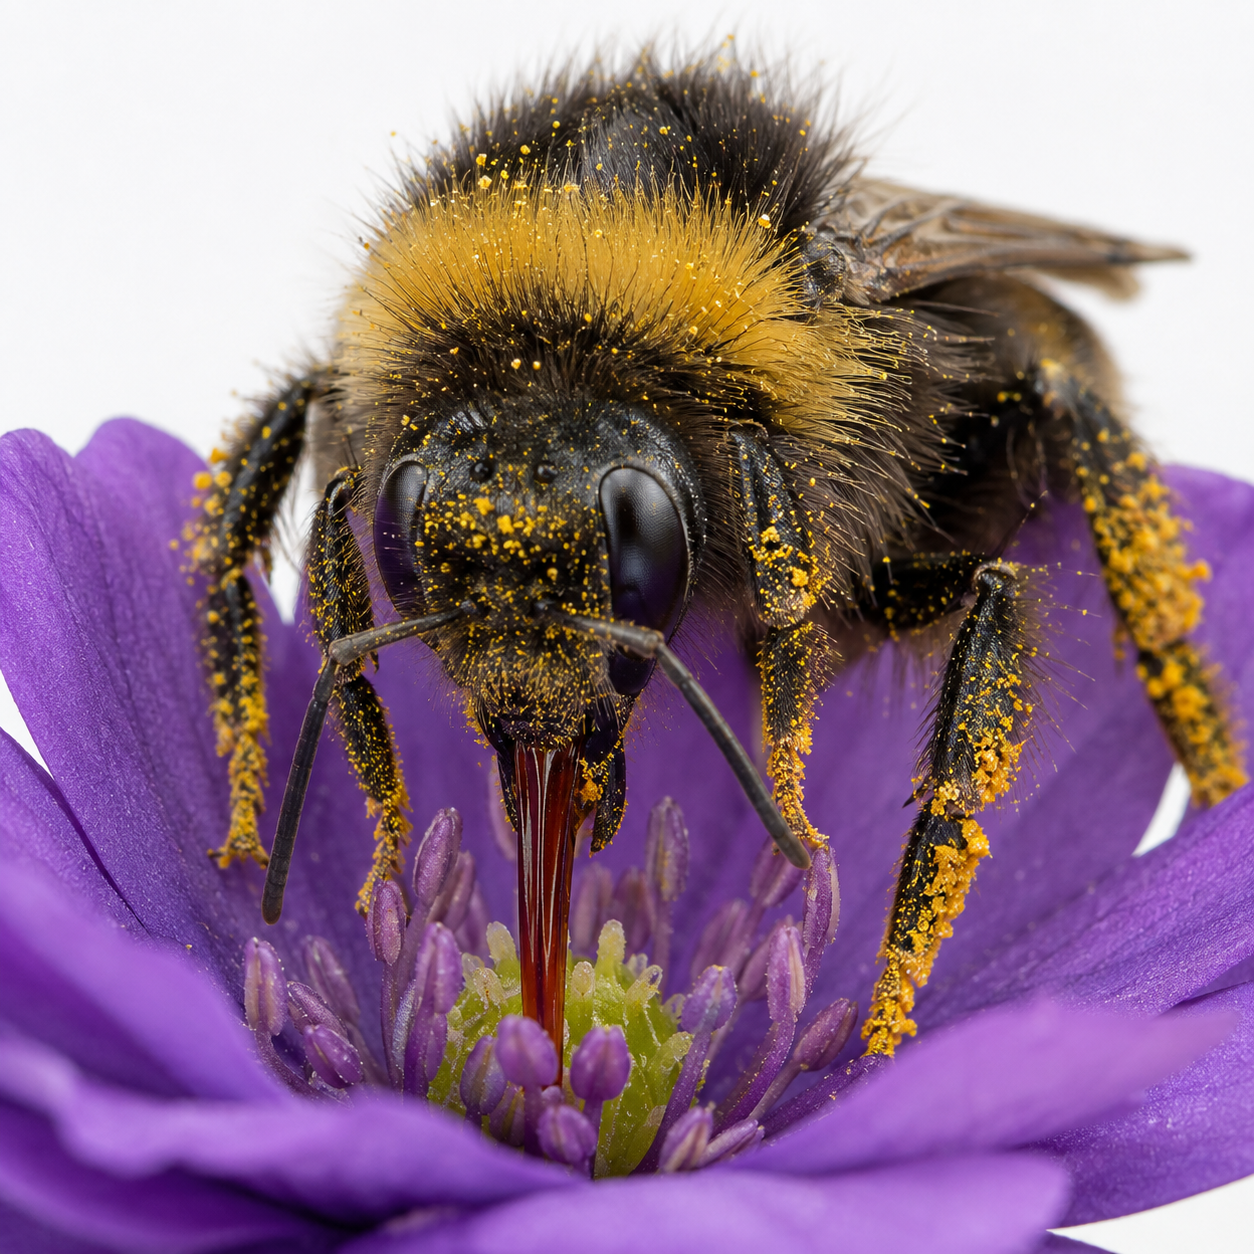
\includegraphics[width=0.56\linewidth]{images/book3/ai/b3-27-bee-flower.png}

{\small \omterm{def:b1:species-interactions:types}{تقايض} في العمل: رحيق للنحلة، ونقل لقاح
للزهرة. وقد شكّل كلٌّ من الشريكين شكلَ الآخر.}
\end{omfigure}

\begin{remark}[المعايشة نادرة وغير مستقرة]\label{rem:b1:species-interactions:commensal}
قليل من التفاعلات $+/0$ حقًا: فالنبات المتعلِّق الذي يظلل مضيفه،
والسمكة اللاصقة التي تكلف قرشها شيئًا من الكبح، وأبو قردان الذي
يأكل ما تثيره الماشية، ليست معايشات إلا بدقة
القياس. فالتفاعلات تُصنَّف بأثرها الصافي،
والأثر الصافي قد يتغير مع الشروط.
\end{remark}

\section{التفاعلات التي تشكّل المجتمع}

\begin{definition}[النوع المفتاح والشلال الغذائي]\label{def:b1:species-interactions:keystone}
\index{نوع مفتاح}\index{شلال غذائي}
\emph{النوع المفتاح} نوع أثره في المجتمع خارج
عن نسبة وفرته أو كتلته الحيوية: فأزله تتغير بنية
المجتمع، وذلك عادة لأنه يتحكم في منافس
سائد. و\emph{الشلال الغذائي} هو انتقال أثر
نازلًا في \omterm{def:b1:ecosystem-organization:foodweb}{سلسلة غذائية} عبر أكثر من مستوى: فحضور مفترس
يخفض آكلات العشب، فترتفع النباتات؛ وإزالته تفعل
العكس. والشلالات تبيّن أن المجتمعات مبنية من الأعلى كما
هي مبنية من الأسفل (بالإنتاجية، \cref{ch:b1:ecosystem-organization}).
\end{definition}

\begin{proposition}[المفترس يستطيع حفظ التنوع]\label{prop:b1:species-interactions:paine}
بأكل النوع الذي كان سيربح المنافسة على المكان أو الموارد لولا
ذلك، يبقي المفترس الخاسرين في المجتمع؛ وإزالته
تدع المنافس السائد يقصيهم، فيهبط التنوع.
\end{proposition}
\begin{proof}[شواهد]
أزال باين (1966) نجم البحر \emph{Pisaster} من امتداد طوله
\qty{8}{m} من شاطئ صخري على ساحل المحيط الهادئ في أمريكا
الشمالية وترك امتدادًا مجاورًا شاهدًا. ونجم البحر يأكل
بلح البحر والبرنقيل وغيرهما من الحيوانات اللاصقة، وبلح البحر بالأفضلية.
وفي غضون سنتين كان بلح البحر \emph{Mytilus} قد انتشر نازلًا على الصخر
وأخذ المكان كله تقريبًا؛ واختفى البرنقيل والكيتونات والبطلينوس
والطحالب التي كانت تعيش في الفجوات، وهبطت الأنواع الخمسة عشر
في القطعة الشاهدة إلى ثمانية. وكانت حصة المفترس نفسه من
الكتلة الحيوية للمجتمع صغيرة؛ لكن إزالته غيّرت كل شيء.
\end{proof}

\begin{omfigure}
\begin{tikzpicture}
\begin{axis}[
  width=0.74\linewidth, height=5.6cm,
  axis x line=bottom, axis y line=left,
  xmin=1963, xmax=1969, ymin=0, ymax=18,
  xlabel={السنة}, ylabel={الأنواع في القطعة},
  xlabel style={font=\small}, ylabel style={font=\small},
  tick label style={font=\small}, xtick={1963,1964,1965,1966,1967,1968},
  x tick label style={/pgf/number format/1000 sep=},
  legend style={font=\scriptsize, at={(0.98,0.03)}, anchor=south east, draw=none, fill=none},
  legend cell align=left,
]
\addplot[omDef, very thick, mark=*] coordinates {(1963,15) (1964,15) (1965,14) (1966,15) (1967,15) (1968,15)};
\addlegendentry{الشاهد: نجم البحر حاضر}
\addplot[omThm, very thick, mark=square*] coordinates {(1963,15) (1964,12) (1965,10) (1966,9) (1967,8) (1968,8)};
\addlegendentry{نجم البحر مزال}
\node[font=\scriptsize, anchor=south west, align=left] at (axis cs:1966.2,10.6) {بلح البحر يأخذ\\ الصخر};
\end{axis}
\end{tikzpicture}

{\small تجربة باين في الإزالة (عن معطياته). التنوع في
القطعة الخالية من المفترس يهبط إلى النصف في خمس سنوات بينما
تحتفظ الشاهدة بأنواعها الخمسة عشر.}
\end{omfigure}

\begin{example}[الذئاب والأيائل والصفصاف]\label{ex:b1:species-interactions:wolves}
أُبيدت الذئاب من متنزه جبلي كبير في عشرينيات القرن العشرين؛
فتكاثرت أيائله ورعت الصفصاف والحور الرجراج على ضفاف
الأنهار حتى الجذوع؛ فتضاءلت القنادس، وهي تحتاج إلى الصفصاف؛ وفقدت
العصافير المغرّدة أدغالها. ولما أُعيدت الذئاب سنة 1995 تراجعت
الأيائل، والأهم أنها تجنبت قيعان الوديان حيث كانت
معرّضة؛ فنما الصفصاف ثانية، وعادت القنادس وبنت سدودًا،
وأعادت الأراضي الرطبة التي صنعتها الأسماكَ والبرمائيات والطيور.
فجرى الشلال من آكل لحم عبر آكل عشب إلى النباتات
ومنها إلى عشرات الأنواع التي لم تلق ذئبًا قط --- مع إسهام
الطقس والصيد ومفترسات أخرى، حتى إن حصة الذئاب من التغير
ما تزال موضع جدل.
\end{example}

\begin{omfigure}
\begin{tikzpicture}[font=\footnotesize, >=Stealth, line cap=round,
  lv/.style={draw, thick, rounded corners=3pt, inner sep=4pt, align=center, fill=white, minimum width=2.6cm}]
  \node[lv, fill=omDef!25] (wolf) at (0,4.5) {ذئاب};
  \node[lv, fill=omProp!20] (elk) at (0,2.8) {أيائل};
  \node[lv, fill=omExo!20] (willow) at (0,1.1) {صفصاف وحور رجراج};
  \node[lv, fill=omProp!20] (beaver) at (3.8,1.1) {قنادس};
  \node[lv, fill=omDef!12] (wet) at (7.4,1.1) {برك وأراضٍ رطبة};
  \node[lv, fill=omThm!15] (birds) at (3.8,-0.6) {عصافير مغرّدة وأسماك\\ وبرمائيات};
  \draw[->, very thick, omThm] (wolf) -- (elk) node[midway, right] {$-$: أقل عددًا، ومبعدة عن ضفاف النهر};
  \draw[->, very thick, omThm] (elk) -- (willow) node[midway, left] {$-$: رعي};
  \draw[->, very thick, omDef] (willow) -- (beaver) node[midway, above=9pt] {$+$: غذاء وسدود};
  \draw[->, very thick, omDef] (beaver) -- (wet) node[midway, above] {$+$};
  \draw[->, very thick, omDef] (willow) -- (birds) node[midway, below left] {$+$};
  \draw[->, very thick, omDef] (wet) |- (birds) node[pos=0.8, below] {$+$};
  \node[anchor=north, align=center, gray] at (3.4,-1.5) {إشارتا سالب تعطيان موجبًا: فعودة الذئاب زادت الصفصاف،\\ والصفصاف حمل الأثر إلى أنواع لم تمسّها الذئاب قط};
\end{tikzpicture}

{\small \omterm{def:b1:species-interactions:keystone}{شلال غذائي}: أثر ينزل ثلاثة مستويات ويمضي
جانبيًا في المجتمع. والإشارات تعطي اتجاه كل
وصلة.}
\end{omfigure}

\begin{omfigure}
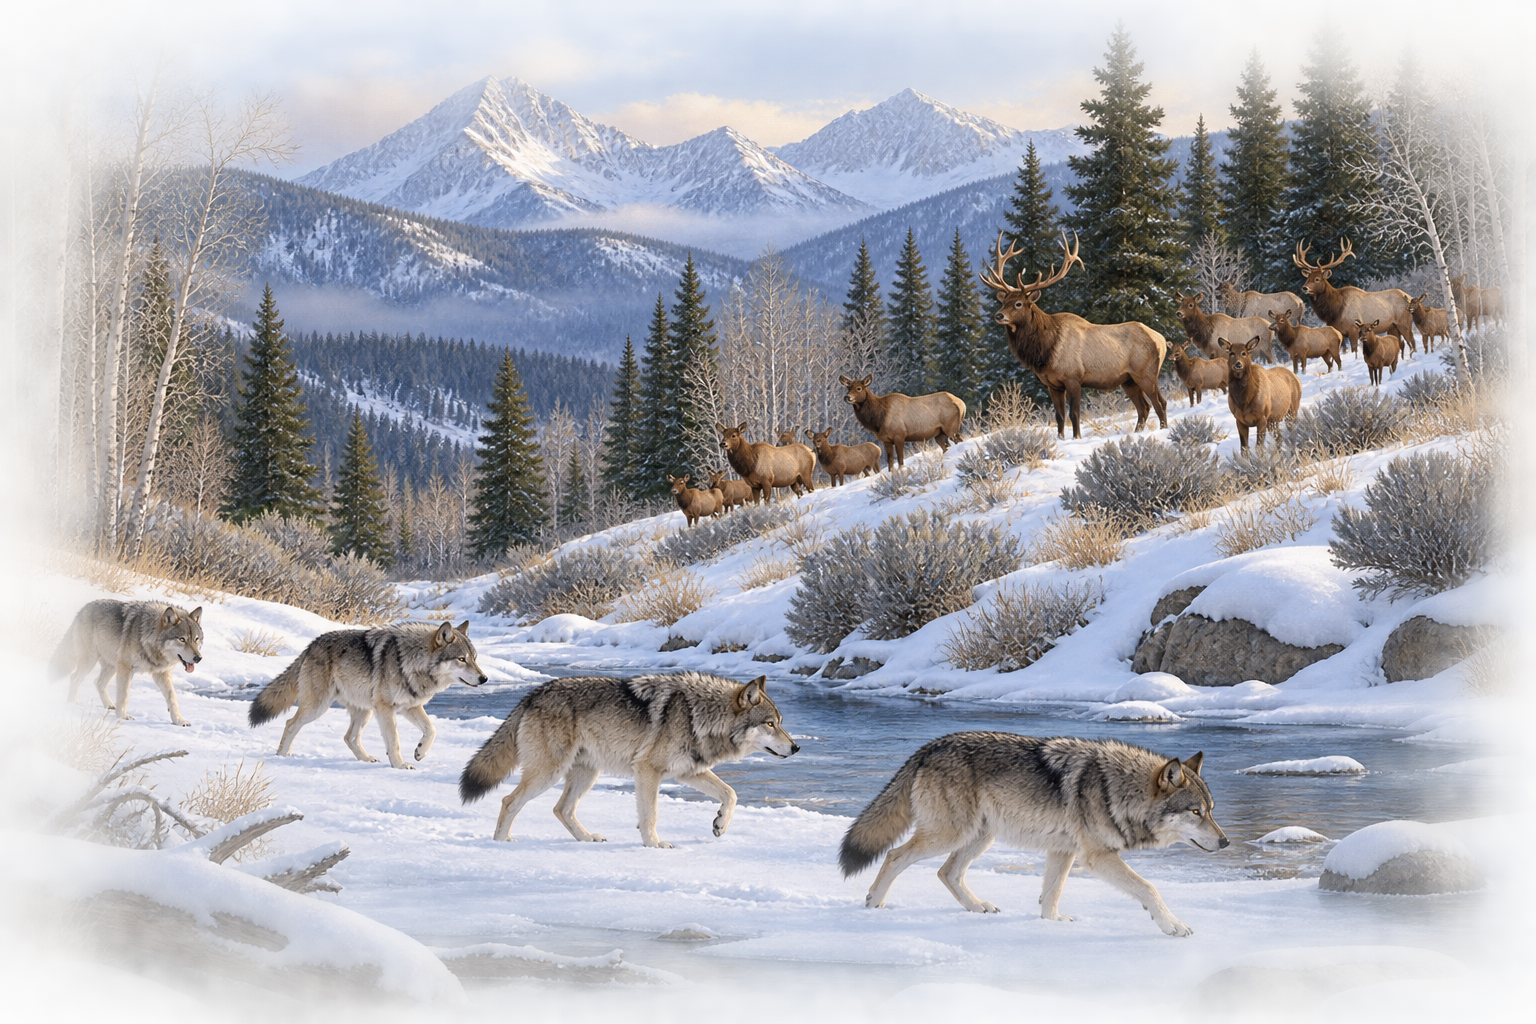
\includegraphics[width=0.6\linewidth]{images/book3/ai/b3-27-wolves-elk.png}

{\small ذئاب وأيائل في وادي نهر في الشتاء. وأثر المفترس
في النبات يجري عبر حيث تجرؤ الأيائل على الرعي بقدر ما
يجري عبر كم عددها.}
\end{omfigure}

\begin{method}[قراءة تفاعل من تجربة]\label{met:b1:species-interactions:reading}
\begin{enumerate}
  \item حدّد التدخل (إزالة، أو إضافة، أو قفص استبعاد،
        أو ازدواج في مزرعة) والشاهد المحفوظ إلى جانبه في
        الشروط نفسها.
  \item قارن، لكل نوع، وفرته بحضور الشريك وبغيابه:
        فإشارة الفرق تعطي إشارة التفاعل على
        ذلك النوع.
  \item ابحث عن الآثار غير المباشرة: فنوع تغيّر دون أن يمسّ
        النوعَ المتدخَّل فيه يقع في نهاية سلسلة ---
        فجد الوسطاء.
  \item تحقق من السلّم الزمني (فقد يستغرق \omterm{def:b1:species-interactions:types}{التنافس} أجيالًا كثيرة
        حتى يُحسم؛ والشلال يجري بسرعة أبطأ مستوى)
        ومن السلّم المكاني (أتصح النتيجة خارج القطعة؟).
  \item طابق النموذج حيث تسمح المعطيات: منحنيات لوجستية
        وخطوط تساوٍ \omterm{def:b1:species-interactions:types}{للتنافس}، \omterm{thm:b1:species-interactions:holling}{ومعادلة الأقراص} \omterm{def:b1:species-interactions:functional}{لاستجابة
        وظيفية}، واقرأ الوسائط من الرسوم المخطَّطة.
\end{enumerate}
\end{method}

\section{تمارين}

\begin{exercise}[$\star$]\label{exo:b1:species-interactions:1}
أعطِ زوج الإشارتين ومثالًا لكل نوع من الأنواع الستة من
التفاعل.
\end{exercise}

\begin{exercise}[$\star$]\label{exo:b1:species-interactions:2}
اذكر مبدأ \omterm{def:b1:species-interactions:competition}{الإقصاء التنافسي} وقل لماذا لا يمنع
خمس هوازج في تنوبة واحدة.
\end{exercise}

\begin{exercise}[$\star$]\label{exo:b1:species-interactions:3}
عرّف \omterm{def:b1:species-interactions:functional}{زمن المعالجة} ومعدل الهجوم، وأعطِ أعظم معدل تغذٍّ
لمفترس عنده $h = \qty{30}{min}$.
\end{exercise}

\begin{exercise}[$\star$]\label{exo:b1:species-interactions:4}
ما \omterm{def:b1:species-interactions:keystone}{النوع المفتاح}؟ ولماذا لا يكون \omterm{def:b1:species-interactions:keystone}{النوع المفتاح} ببساطة
الأوفر عددًا؟
\end{exercise}

\begin{exercise}[$\star\star$]\label{exo:b1:species-interactions:5}
النوع 1 عنده $K_1 = 500$، والنوع 2 عنده $K_2 = 400$، مع $\alpha =
0.5$ و$\beta = 0.6$. ارسم \omterm{prop:b1:species-interactions:lotka}{خطي التساوي} وأعطِ النتيجة.
وأعد الرسم عند $\alpha = 2$ و$\beta = 0.6$.
\end{exercise}

\begin{exercise}[$\star\star$]\label{exo:b1:species-interactions:6}
مفترس عنده $a = \qty{0.2}{m^2/h}$ و$h = \qty{0.25}{h}$ يلقى
فرائس عند \qty{10}{} وعند \qty{100}{} في المتر المربع. احسب
معدل تغذّيه في كل حالة والكثافة التي يكون عندها نصف
مشبع.
\end{exercise}

\begin{exercise}[$\star\star$]\label{exo:b1:species-interactions:7}
لماذا تثبّت استجابة النمط III \omterm{def:b1:populations:population}{جمهرة} فريسة عند كثافة
منخفضة بينما لا تثبّتها استجابة النمط II؟
\end{exercise}

\begin{exercise}[$\star\star$]\label{exo:b1:species-interactions:8}
من تجربة غوز، فسّر لماذا تعايش \emph{P.~bursaria}
مع \emph{P.~aurelia} ولم يتعايش \emph{P.~caudatum}. فما الذي صنع
الفرق: معدل النمو أم \omterm{def:b1:ecosystem-organization:niche}{المكانة}؟
\end{exercise}

\begin{exercise}[$\star\star$]\label{exo:b1:species-interactions:9}
محاكٍ بيتسي يصير أوفر من نموذجه السام. تنبأ
بما يحدث لحماية كليهما، ولماذا يكون نجاح المحاكي
محدودًا ذاتيًا.
\end{exercise}

\begin{exercise}[$\star\star\star$]\label{exo:b1:species-interactions:10}
فقدت قطعة باين المزال منها المفترس سبعة أنواع. فسّر، بنموذج \omterm{prop:b1:species-interactions:lotka}{خطي
التساوي}، كيف يحوّل مفترس يأكل المنافس السائد
إقصاءً إلى تعايش.
\end{exercise}

\begin{exercise}[$\star\star\star$]\label{exo:b1:species-interactions:11}
فطر ميكوريزي يأخذ \qty{15}{\%} من نواتج التركيب الضوئي في نبات
ويمده بنسبة \qty{80}{\%} من فوسفاته. ففي أي شروط يكون الارتباط
تقايضًا، وفي أي شروط تطفلًا؟ واقترح تجربة للتمييز.
\end{exercise}

\begin{exercise}[$\star\star\star$]\label{exo:b1:species-interactions:12}
صمّم تجربة لاختبار ما إذا كانت الذئاب، لا الطقس ولا الصيد، هي
سبب تعافي الصفصاف: الشواهد، والمكررات،
والمتغيرات المقيسة، وأي نتيجة تدحض الشلال.
\end{exercise}

\section{مسألة: المفترس والشاطئ}

\begin{problem}[{مسألة نهاية الأسبوع --- هدبيات غوز في أنبوب،
ومعطيات تغذّي مفترس تُطابَق بمعادلة الأقراص، وشاطئ باين
بنجم بحره وبدونه، وميزانية ملقِّح، وختامًا معدل الهجوم
وزمن المعالجة عند المفترس}]
\label{pb:b1:species-interactions:1}

\medskip
\noindent\textbf{الجزء الأول --- \omterm{def:b1:species-interactions:types}{التنافس} في أنبوب.}
يُنمّى نوعان من الهدبيات كل واحد وحده: فالنوع A يبلغ $K_A = 200$ في
\qty{0.5}{mL} عند $r_A = \qty{0.8}{d^{-1}}$؛ والنوع B يبلغ
$K_B = 130$ عند $r_B = \qty{0.55}{d^{-1}}$. ومعًا، يستعمل فرد
من B من الغذاء قدر ما يستعمله $\alpha = 1.4$ من A، وفرد من A
قدر ما يستعمله $\beta = 0.9$ من B.
\begin{enumerate}
  \item اكتب \omterm{prop:b1:species-interactions:lotka}{خطي التساوي} وتقاطعيهما مع المحورين.
  \item ارسمهما واذكر أي النوعين يفوز، ولماذا لا تتوقف النتيجة
        على الأعداد الابتدائية.
  \item من زمني التضاعف ($\ln 2/r$)، أي النوعين كنت تتوقع أن
        يفوز من معدل النمو وحده؟
  \item نوع ثالث C يتغذى في قاع الأنبوب وينافس
        A منافسة ضعيفة فقط ($\alpha = 0.3$ و$\beta = 0.3$ و$K_C = 100$).
        ارسم \omterm{prop:b1:species-interactions:lotka}{خطي التساوي} وأعطِ النتيجة.
  \item لماذا يصح مبدأ الإقصاء في أنبوب ويخفق كثيرًا
        في غابة؟ أعطِ سببين.
  \item احسب عددي A وC عند التوازن من تقاطع
        \omterm{prop:b1:species-interactions:lotka}{خطي التساوي}.
\end{enumerate}

\medskip
\noindent\textbf{الجزء الثاني --- \omterm{thm:b1:species-interactions:holling}{معادلة الأقراص}.}
تُعرض على خنفساء مفترسة فرائس بكثافات 5 و10 و20 و40 و
80 في المتر المربع؛ فتأكل 2.0 و3.3 و5.0 و6.7 و8.0 فريسة في اليوم
على الترتيب.
\begin{enumerate}[resume]
  \item ارسم معدل التغذّي في مقابل الكثافة وحدّد نمط
        الاستجابة.
  \item احسب $1/f$ و$1/N$ لكل نقطة وارسمهما.
  \item من الميل والتقاطع، استخرج $a$ و$h$.
  \item احسب أعظم معدل تغذٍّ وكثافة نصف
        الإشباع.
  \item عند أي من الكثافات الخمس تنفق الخنفساء أكثر
        من نصف وقتها في المعالجة؟
  \item تنمو فرائس الخنفساء نموًا لوجستيًا عند $r = \qty{0.1}{d^{-1}}$
        و$K = 200$. فعند أي كثافة يساوي نمو الفريسة (في المتر
        المربع الخالي من الخنافس) استهلاكَ الخنفساء إذا كانت
        هناك خنفساء واحدة في المتر المربع؟ وهل هذا التوازن
        مستقر أمام ارتفاع صغير في الفريسة؟
  \item يظهر نوع فريسة ثانٍ تعالجه الخنفساء أسرع
        مرتين. تنبأ بتغير مدخول الخنفساء الكلي عند الكثافة
        العالية.
\end{enumerate}

\medskip
\noindent\textbf{الجزء الثالث --- الشاطئ.}
في قطعة باين الشاهدة كان في المجتمع 15 نوعًا؛ وفي قطعة
الإزالة هبط العدد 15 و12 و10 و9 و8 و8 على مدى خمس سنوات، وارتفعت
تغطية بلح البحر للصخر من \qty{20}{\%} إلى \qty{85}{\%}.
\begin{enumerate}[resume]
  \item احسب \omterm{def:b1:ecosystem-organization:diversity}{دليل شانون} لقطعة فيها 15 نوعًا بوفرة
        متساوية، ولقطعة فيها 8 أنواع يكون فيها بلح البحر
        \qty{85}{\%} من الأفراد وتتقاسم السبعة الأخرى الباقي
        بالتساوي.
  \item بأي معامل هبط التنوع؟
  \item فسّر، بإشارات التفاعلات، لماذا قوّت إزالة تفاعل
        $+/-$ (\omterm{def:b1:species-interactions:types}{الافتراس} على بلح البحر) تفاعلًا $-/-$
        (\omterm{def:b1:species-interactions:types}{التنافس} على الصخر).
  \item كان نجم البحر أقل من \qty{1}{\%} من كتلة القطعة الحيوية.
        فلماذا تكون الكتلة الحيوية دليلًا رديئًا على أهمية النوع؟
  \item تنبأ بما كان سيحدث لو كانت فريسة نجم البحر المفضلة
        أندر الأنواع لا أسودها.
  \item اقترح طريقة لتأكيد أن السبب كان \omterm{def:b1:species-interactions:types}{الافتراس} على بلح البحر
        لا أثرًا آخر لنجم البحر (تجربة أقفاص).
\end{enumerate}

\medskip
\noindent\textbf{الجزء الرابع --- ميزانية \omterm{def:b1:species-interactions:types}{تقايض}.}
تزور نحلة 1000 زهرة في اليوم وتجمع \qty{40}{mg} من السكر؛
وتعطي كل زهرة \qty{40}{\micro g} من السكر في الرحيق وتتلقى
لقاحًا من 3 أزهار سابقة وسطيًا في كل زيارة. وتنفق النبتة
\qty{1}{\%} من نواتج تركيبها الضوئي اليومية (\qty{4}{mg} من السكر لكل
زهرة) على الرحيق؛ ويكلف طيران النحلة \qty{0.5}{mg} من السكر في
الساعة من الاعتلاف (\qty{8}{h}).
\begin{enumerate}[resume]
  \item احسب كسب النحلة الصافي من السكر في اليوم ومكافئه
        الطاقي عند \qty{16}{kJ/g}.
  \item احسب كلفة النبتة اليومية لكل زهرة ككسر من
        نواتج تركيبها الضوئي وقل ماذا تشتري بها.
  \item لماذا يكون هذا التفاعل $+/+$ مع أن كل شريك
        يستغل الآخر؟
  \item سارق رحيق يعضّ \omterm{def:b1:nucleic-acids:nucleotide}{قاعدة} الزهرة ويأخذ
        الرحيق دون أن يمسّ اللقاح. أعطِ إشارتي تفاعل
        السارق مع النبتة وأثره المرجح في النحلة.
  \item ارسم مخطط الإشارات للنبتة والنحلة والسارق وطائر
        يأكل السارقين، وتنبأ بالأثر غير المباشر للطائر في
        النبتة.
  \item اذكر النتيجة: معدل الهجوم \omterm{def:b1:species-interactions:functional}{وزمن المعالجة} عند
        الخنفساء، وأعظم معدل تغذٍّ لها.
\end{enumerate}
\end{problem}
